\documentclass[]{article}
\usepackage{lmodern}
\usepackage{amssymb,amsmath}
\usepackage{ifxetex,ifluatex}
\usepackage{fixltx2e} % provides \textsubscript
\ifnum 0\ifxetex 1\fi\ifluatex 1\fi=0 % if pdftex
  \usepackage[T1]{fontenc}
  \usepackage[utf8]{inputenc}
\else % if luatex or xelatex
  \ifxetex
    \usepackage{mathspec}
  \else
    \usepackage{fontspec}
  \fi
  \defaultfontfeatures{Ligatures=TeX,Scale=MatchLowercase}
\fi
% use upquote if available, for straight quotes in verbatim environments
\IfFileExists{upquote.sty}{\usepackage{upquote}}{}
% use microtype if available
\IfFileExists{microtype.sty}{%
\usepackage[]{microtype}
\UseMicrotypeSet[protrusion]{basicmath} % disable protrusion for tt fonts
}{}
\PassOptionsToPackage{hyphens}{url} % url is loaded by hyperref
\usepackage[unicode=true]{hyperref}
\hypersetup{
            pdftitle={Snow crab simulations: effects of bycatch in the groundfish fisheries},
            pdfauthor={Cody Szuwalski},
            pdfborder={0 0 0},
            breaklinks=true}
\urlstyle{same}  % don't use monospace font for urls
\usepackage[margin=1in]{geometry}
\usepackage{longtable,booktabs}
% Fix footnotes in tables (requires footnote package)
\IfFileExists{footnote.sty}{\usepackage{footnote}\makesavenoteenv{long table}}{}
\usepackage{graphicx,grffile}
\makeatletter
\def\maxwidth{\ifdim\Gin@nat@width>\linewidth\linewidth\else\Gin@nat@width\fi}
\def\maxheight{\ifdim\Gin@nat@height>\textheight\textheight\else\Gin@nat@height\fi}
\makeatother
% Scale images if necessary, so that they will not overflow the page
% margins by default, and it is still possible to overwrite the defaults
% using explicit options in \includegraphics[width, height, ...]{}
\setkeys{Gin}{width=\maxwidth,height=\maxheight,keepaspectratio}
\IfFileExists{parskip.sty}{%
\usepackage{parskip}
}{% else
\setlength{\parindent}{0pt}
\setlength{\parskip}{6pt plus 2pt minus 1pt}
}
\setlength{\emergencystretch}{3em}  % prevent overfull lines
\providecommand{\tightlist}{%
  \setlength{\itemsep}{0pt}\setlength{\parskip}{0pt}}
\setcounter{secnumdepth}{0}
% Redefines (sub)paragraphs to behave more like sections
\ifx\paragraph\undefined\else
\let\oldparagraph\paragraph
\renewcommand{\paragraph}[1]{\oldparagraph{#1}\mbox{}}
\fi
\ifx\subparagraph\undefined\else
\let\oldsubparagraph\subparagraph
\renewcommand{\subparagraph}[1]{\oldsubparagraph{#1}\mbox{}}
\fi

% set default figure placement to htbp
\makeatletter
\def\fps@figure{htbp}
\makeatother

\pagenumbering{gobble}

\title{Snow crab simulations: effects of bycatch in the groundfish fisheries}
\author{Cody Szuwalski}
\date{July 2020}

\begin{document}
\maketitle

{
\setcounter{tocdepth}{3}
\tableofcontents
}
\newpage

\newpage

\section{Introduction}\label{introduction}

Sarah Marrinan and Sara Cleaver (North Pacific Fishery Management
Council staff) presented information to the Crab Plan Team at its May
2020 meeting on a proposed Council action to change crab PSC (Prohibited
Species Catch) limits in the groundfish fisheries to the lowest possible
level when the directed crab fishery is closed. There are currently area
PSC limits in place for Bristol Bay red king crab, Tanner crab, and snow
crab for groundfish vessels using trawl gear. The current limits are
rarely exceeded, and even if they were set at the lowest level would
rarely be constraining. Council staff asked the CPT about the importance
of bycatch in crab population dynamics. Currently there is very little
crab bycatch in groundfish fisheries compared to the directed fisheries.
However, it was noted that there is very little information on the
unobserved mortality of crab species. Thus, Council staff asked if
assessment authors could examine the effects of increased bycatch on
model results. Consequently, the Crab Plan Team (CPT) requested at its
May 2020 meeting that:

``Assessment authors should rerun the assessments for BBRKC, Tanner
crab, and snow crab with higher assumed levels of bycatch abundance
(increases of 50\% and 100\%) as a sensitivity analysis. These should be
provided to Council staff within the next two months for inclusion in
the October Council document.''

This report addresses this request for snow crab.

\section{Methods}\label{methods}

The methodology implemented here departs slightly from what the CPT
requestions. Following, Buck Stockhausen's example, the model was rerun
with three bycatch scenarios in which historical bycatch was 50\%,
100\%, and 1000\% larger. In these simulations, all parameters governing
biological processes (e.g.~recruitment, natural mortality, growth,
maturity) were specified to the values estimated in the 2019 assessment.
Most parameters governing fisheries processes (directed and discard
fishing mortality and directed, discard, and bycatch selectivity) were
also fixed. Only fishing mortality associated with bycatch in other
fisheries (which is primarily trawl fisheries for snow crab) was
estimated to accommodate the newly input bycatch numbers.

\section{Results}\label{results}

Increases in bycatch resulted in a general scaling down of mature male
biomass (MMB) at the time of the survey (\autoref{mmbfits}). Females
were not affected because the selectivity of the bycatch `fleet' in the
model generally excludes them from mortality (\autoref{predfmort}). The
associated estimated fishing mortality increased predictably with
increases in the input bycatch (\autoref{predfmort}).

The translation of these changes to most management quantities was also
predictable (\autoref{stepchange}). Terminal year MMB did not
appreciably because the magnitude of bycatch relative to MMB is very
small. B35 did not change because the biological processes determining
it were fixed. F35 decreased as bycatch levels increased becaues F35 is
only related to the directed fishery. As the `expected' by catch
increases (which is determined by input levels), the fishing mortality
allowed in the directed fishery has to decrease to compensate.

The changes in the overfishing level (OFL) were less intuitive. As
bycatch increased, the OFL also increased. The OFL is calculated as the
sum of the retained catch and mortality associated with discards in the
directed fishery and bycatch elsewhere. So, the decreases in the
retained portion of the OFL resulting from decreases in the FOFL (which
themselves are the result of increases in bycatch) are outpaced by the
increases in the portion of the OFL allocated to bycatch.

The reason this occurs is related to the selectivity of the bycatch--a
fraction of the bycatch is not mature (\autoref{predfmort}). The harvest
control rule only considers mature male biomass when calculating the
FOFL (and OFL), but the F allocated for bycatch is fixed and does not
consider the amount of MMB (or immature biomass) available. So, as the F
allocated to bycatch increases, increases in the contribution of bycatch
to the OFL that is immature are possible. Increases in the amount of
immature crab caught do not impact the MMB, so the OFL can increase as
bycatch increases without impacting the `status' of the fishery. This
issue could be exacerbated by the large recruitment class coming through
the population.

\section{Discussion}\label{discussion}

Based on these analyses, changes in the amount of bycatch observed would
have had the largest impact during the period when bycatches were
largest (e.g.~the mid 1990s through the mid 2010s). In the most recent
years, bycatch has been so small that inputting even 10 times the amount
of bycatch reported resulted in very small changes to the terminal year
of MMB.

Increases in the OFL

Maybe need to reconsider the way immature bycatch is treated in the
harvest control rule.

\newpage

\begin{figure}
\centering
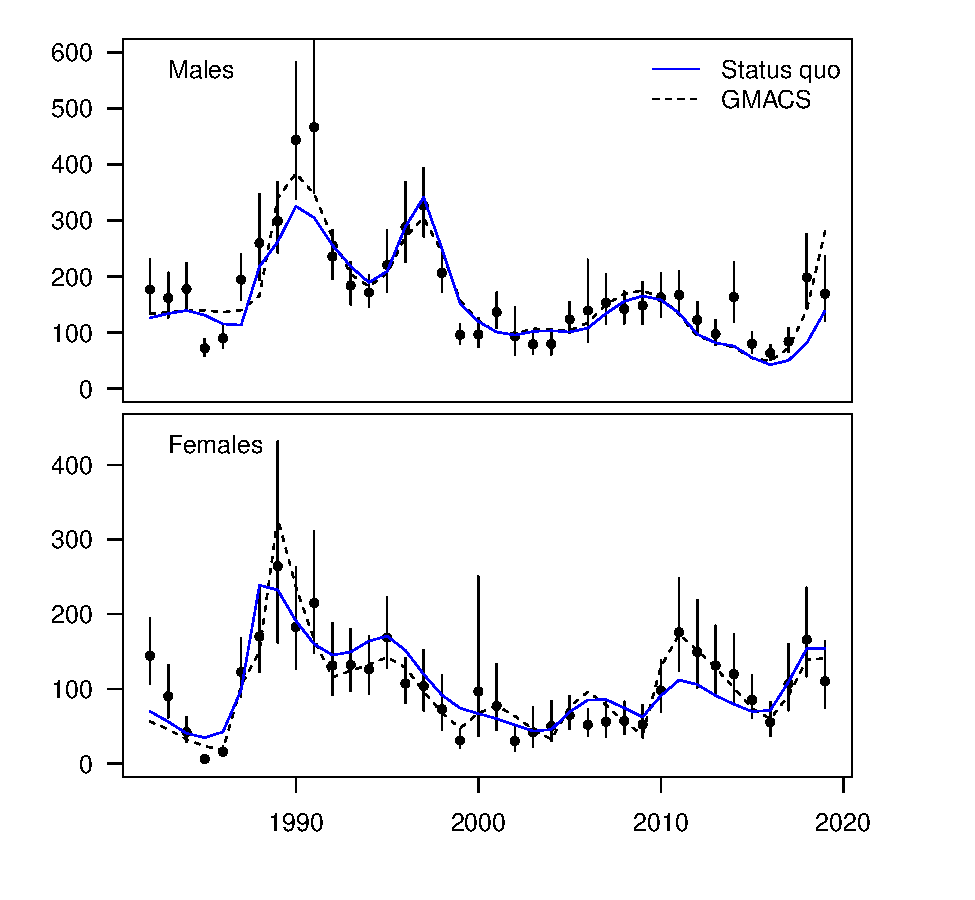
\includegraphics{PSC_snow_files/figure-latex/unnamed-chunk-3-1.pdf}
\caption{\label{mmbfits}Model fits to the observed mature biomass at
survey}
\end{figure}

\newpage

\begin{figure}
\centering
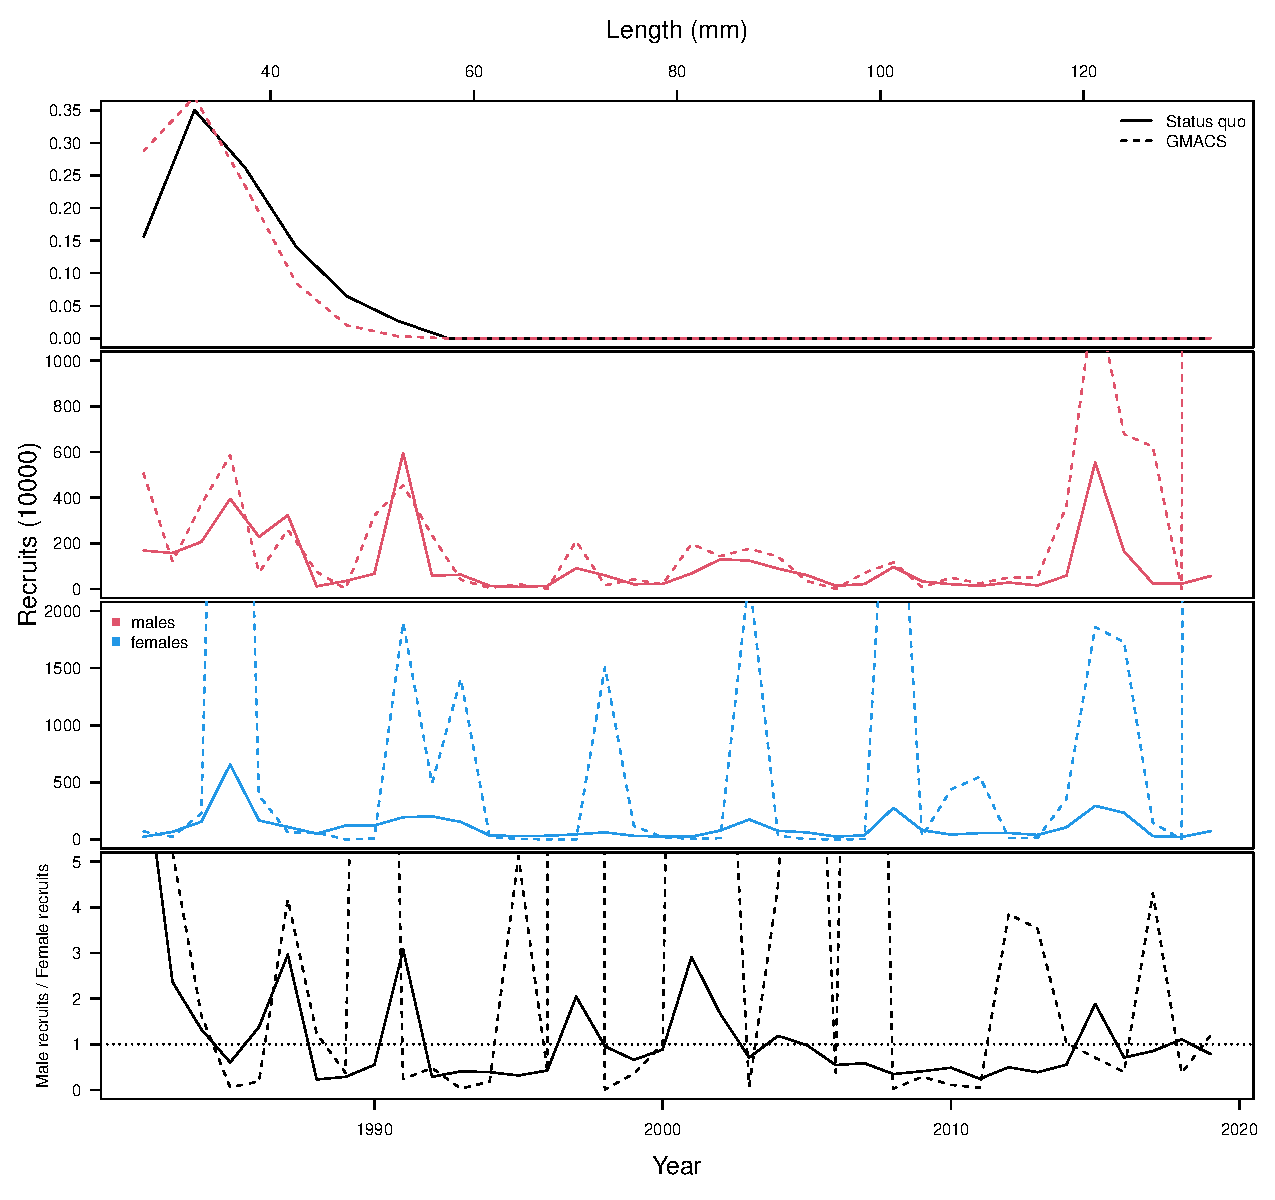
\includegraphics{PSC_snow_files/figure-latex/unnamed-chunk-4-1.pdf}
\caption{\label{predfmort}Model predicted fishing mortalities and
selectivities for all sources of mortality}
\end{figure}

\newpage

\begin{longtable}[]{@{}lccccc@{}}
\caption{\label{stepchange}Changes in management quantities for each
scenario considered. Reported management quantities are derived from
maximum likelihood estimates.}\tabularnewline
\toprule
\begin{minipage}[b]{0.17\columnwidth}\raggedright\strut
Model\strut
\end{minipage} & \begin{minipage}[b]{0.09\columnwidth}\centering\strut
MMB\strut
\end{minipage} & \begin{minipage}[b]{0.09\columnwidth}\centering\strut
B35\strut
\end{minipage} & \begin{minipage}[b]{0.09\columnwidth}\centering\strut
F35\strut
\end{minipage} & \begin{minipage}[b]{0.09\columnwidth}\centering\strut
FOFL\strut
\end{minipage} & \begin{minipage}[b]{0.09\columnwidth}\centering\strut
OFL\strut
\end{minipage}\tabularnewline
\midrule
\endfirsthead
\toprule
\begin{minipage}[b]{0.17\columnwidth}\raggedright\strut
Model\strut
\end{minipage} & \begin{minipage}[b]{0.09\columnwidth}\centering\strut
MMB\strut
\end{minipage} & \begin{minipage}[b]{0.09\columnwidth}\centering\strut
B35\strut
\end{minipage} & \begin{minipage}[b]{0.09\columnwidth}\centering\strut
F35\strut
\end{minipage} & \begin{minipage}[b]{0.09\columnwidth}\centering\strut
FOFL\strut
\end{minipage} & \begin{minipage}[b]{0.09\columnwidth}\centering\strut
OFL\strut
\end{minipage}\tabularnewline
\midrule
\endhead
\begin{minipage}[t]{0.17\columnwidth}\raggedright\strut
Status quo\strut
\end{minipage} & \begin{minipage}[t]{0.09\columnwidth}\centering\strut
105\strut
\end{minipage} & \begin{minipage}[t]{0.09\columnwidth}\centering\strut
123.1\strut
\end{minipage} & \begin{minipage}[t]{0.09\columnwidth}\centering\strut
1.771\strut
\end{minipage} & \begin{minipage}[t]{0.09\columnwidth}\centering\strut
1.771\strut
\end{minipage} & \begin{minipage}[t]{0.09\columnwidth}\centering\strut
51.31\strut
\end{minipage}\tabularnewline
\begin{minipage}[t]{0.17\columnwidth}\raggedright\strut
1.5x bycatch\strut
\end{minipage} & \begin{minipage}[t]{0.09\columnwidth}\centering\strut
105\strut
\end{minipage} & \begin{minipage}[t]{0.09\columnwidth}\centering\strut
123.1\strut
\end{minipage} & \begin{minipage}[t]{0.09\columnwidth}\centering\strut
1.765\strut
\end{minipage} & \begin{minipage}[t]{0.09\columnwidth}\centering\strut
1.765\strut
\end{minipage} & \begin{minipage}[t]{0.09\columnwidth}\centering\strut
51.39\strut
\end{minipage}\tabularnewline
\begin{minipage}[t]{0.17\columnwidth}\raggedright\strut
2x bycatch\strut
\end{minipage} & \begin{minipage}[t]{0.09\columnwidth}\centering\strut
105\strut
\end{minipage} & \begin{minipage}[t]{0.09\columnwidth}\centering\strut
123.1\strut
\end{minipage} & \begin{minipage}[t]{0.09\columnwidth}\centering\strut
1.76\strut
\end{minipage} & \begin{minipage}[t]{0.09\columnwidth}\centering\strut
1.76\strut
\end{minipage} & \begin{minipage}[t]{0.09\columnwidth}\centering\strut
51.46\strut
\end{minipage}\tabularnewline
\begin{minipage}[t]{0.17\columnwidth}\raggedright\strut
10x bycatch\strut
\end{minipage} & \begin{minipage}[t]{0.09\columnwidth}\centering\strut
104.9\strut
\end{minipage} & \begin{minipage}[t]{0.09\columnwidth}\centering\strut
123.1\strut
\end{minipage} & \begin{minipage}[t]{0.09\columnwidth}\centering\strut
1.697\strut
\end{minipage} & \begin{minipage}[t]{0.09\columnwidth}\centering\strut
1.697\strut
\end{minipage} & \begin{minipage}[t]{0.09\columnwidth}\centering\strut
52.42\strut
\end{minipage}\tabularnewline
\bottomrule
\end{longtable}

\newpage

\end{document}
